\documentclass{sig-alternate}

\begin{document}
	\title{CSCI-620 Data Mining with the Airbnb Dataset}
	\subtitle{[Exploring and Mining the dataset of NY Airbnbs]}
	
	\numberofauthors{4}
	\author
	{
		\alignauthor
		Aishwarya Rao
		\email{ar2711@rit.edu}
		\alignauthor
		Apurav Khare
		\email{ak2816@rit.edu}
		\and
		\alignauthor
		Martin Qian
		\email{jq3513@rit.edu}
		\alignauthor
		Prateek Kalasannavar
		\email{pk6685@rit.edu}
	}
	
	\maketitle
	\begin{abstract}
		
		The project aims to create a prediction model on the New York Airbnb Dataset that is capable of predicting which price group a particular house falls into. The approach we use is to build a classification model (such as decision tree) to predict a discrete version of the price (For instance, expensive vs cheap). One of the deliverable this project will include is determining what factors affect the price.   
		
	\end{abstract}
	
	\section{Current progress}
	
	\subsection{The Data Mining task}
	As mentioned in the previous phase, the data mining task selected was to build a classification model that is capable of predicting the price group a listing would fall into. This decision is based on a number of reasons. One, a model capable of predicting the price of a new listing has real-world applications. A landlord looking to put up a listing for a new house in New York would be able to use this model to determine the expected range of prices for his house and price it accordingly to make the most profit. Two, the exploration of the dataset revealed that there are a number of attributes in the data that correlate to the price. This indicates that these attributes do help determine the price and validates our hypothesis that the price can be predicted reasonably well by a data mining algorithm. Figure \ref{corr} depicts the correlation of some of the attributes with the price, which will help choose the right features for the model. 
	\begin{figure}[ht]
		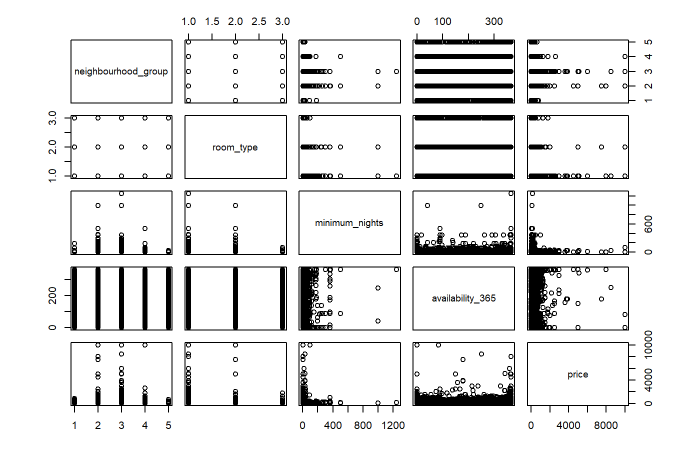
\includegraphics[width=8cm]{corr.png}
		\centering
		\caption{Correlation of price between other attributes}
		\label{corr}
	\end{figure}
	
	\subsection{Categorizing Price}
	Price the New York Airbnb Dataset is a continuous attribute with the following details - \newline
	 Min.   :    0.0  \newline
	1st Qu.:   69.0  \newline
	Median :  106.0  \newline
	Mean   :  152.7  \newline
	3rd Qu.:  175.0  \newline
	Max.   :10000.0  \newline
	To perform a classification task on the price, this attribute has to be made categorical. We used quartiles to create four different classes ranging from cheap to expensive. The quartiles were as follows,
	Category 1 : 0 - 25\% (0- 69) \newline
	Category 2 : 26 - 50\% (70 -106) \newline
	Category 3 : 50 - 75\% (107- 175) \newline
	Category 4 : 75 - 100\% (176- 10000) \newline
	Figure \ref{dist} shows the distribution of the data after the categorical split. As seen below, the distribution is well balanced with all classes having approximately the same number of instances, eliminating any class skewed dataset problems.
	\begin{figure}[ht]
		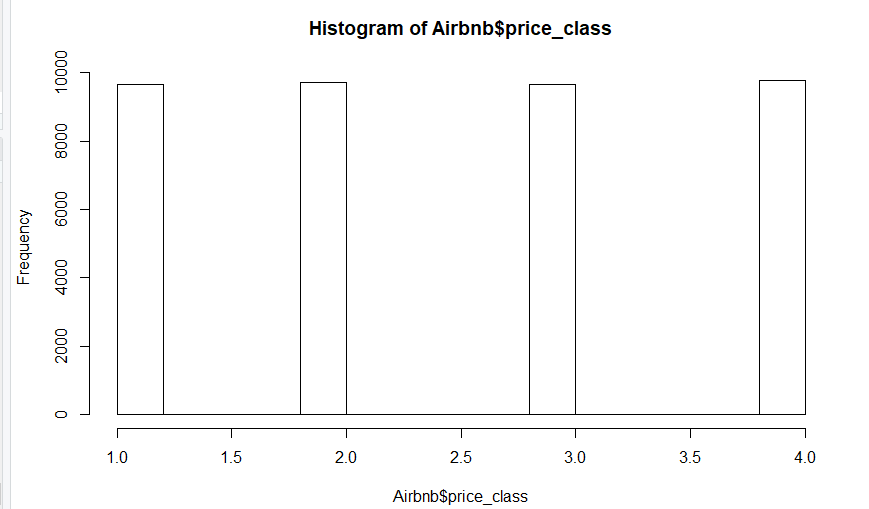
\includegraphics[width=8cm]{dist.png}
		\caption{Distribution of price after categorizing}
		\label{dist}
		\centering
	\end{figure}
	\subsection{Cleaning the dataset}
	\subsection{Feature Engineering} 
	\subsection{Train and test split}
	\subsection{Basic model}
	\subsection{Evaluation metrics}
	\section{Future work} 
	
	
\end{document}
